\section{Thermalization: The Elastic Case}

\begin{frame}{Kinetic Evolution dominated by Elastic Collisions I}
\vspace{0.5em}
Elastic collisions conserve \alert{particle number} $\longrightarrow$ Introduce chemical potential $\mu$\\[0.5em]

\begin{itemize}
	\item Phase space distribution function given by \alert{Bose-Einstein distribution}:
\end{itemize}
\begin{equation}
	f_{\mathrm{eq}}(\mathbf{k}) = \frac{1}{\exp(\frac{\omega_{\mathbf{k}}-\mu}{T}) - 1}
\end{equation}

\begin{itemize}
	\item The energy density and the number density then read
\end{itemize}
\begin{align}
	\varepsilon_{\mathrm{eq}} &=\int_{\mathbf{p}} \omega_{\mathbf{p}}\cdot f_{\mathrm{eq}}(\mathbf{p}) \\
	n_{\mathrm{eq}} &= \int_{\mathbf{p}} 	f_{\mathrm{eq}}(\mathbf{p})
\end{align}
\begin{itemize}
	\item \alert{Remark:} Due to many-body interactions, the gluons can develop an effective medium dependent mass with 
\end{itemize}
\begin{equation}
	m_0^2 \sim \alpha_{\mathrm{s}}\int_{\mathbf{p}}\frac{\dd f_0}{\dd\omega_{\mathbf{p}}} \sim Q_{\mathrm{s}}^2 \qquad (\text{cf.}\ m_{\mathrm{eq}}\sim \alpha_{\mathrm{s}}^{1/2}T \sim \alpha_{\mathrm{s}}^{1/4}Q_{\mathrm{s}})
\end{equation}\label{eqn:bose-einstein}
\end{frame}

\begin{frame}{Kinetic Evolution dominated by Elastic Collisions II}
\begin{itemize}
	\item The mass $m$ defines an upper bound on the number density:
\end{itemize}
\begin{equation}
	n_{\mathrm{max}} = \int\frac{\dd[3]\mathbf{k}}{(2\pi)^3}\frac{1}{\exp\left(\frac{\omega_{\mathbf{k}}-m_0}{T}\right)-1}\sim T^{\phantom{.}3} \quad\qquad (m\ll T\phantom{.})
\end{equation}
\begin{itemize}
	\item This observation yields the statement, that $n_{\mathrm{max}} \sim Q_{\mathrm{s}}^3/\alpha_{\mathrm{s}}^{3/4}$ is smaller than the initial density  $n_0 \sim Q_{\mathrm{s}}^3/\alpha_{\mathrm{s}}$.
	\item \alert{Interpretation:} When we consider only elastic collisions, the gluons form a \alert{Bose-Einstein condensate} (BEC) with distribution function
\begin{equation}
	f_{\mathrm{eq}}(\mathbf{k}) = n_c\cdot\delta(\mathbf{k}) + \frac{1}{\exp\left(\frac{\omega_{\mathbf{k}}-m_0}{T}\right)-1}
\end{equation}
	with 
	\begin{equation}
	 n_c \sim  \frac{Q_{\mathrm{s}}^3}{\alpha_{\mathrm{s}}}\left(1-\alpha_{\mathrm{s}}^{1/4}\right)  \qquad (\text{note}\ n_c\cdot m \sim \alpha_{\mathrm{s}}^{1/4}T^{\phantom{.}4} \ll \varepsilon_0)
\end{equation}
\end{itemize}
\end{frame}

\begin{frame}{BEC: A short Reminder (and Teaser)}
\vspace{0.5em}
What is a Bose-Einstein Condensate?\\[0.5em]

\begin{itemize}
	\item Bosons are allowed to share the same quantum state.
	\item At very low temperatures the occupation of the lowest quantum state rises extremely fast. 
	\item New \enquote{state of matter} has extremely interesting properties. 
\end{itemize}
\begin{figure}
	\centering
	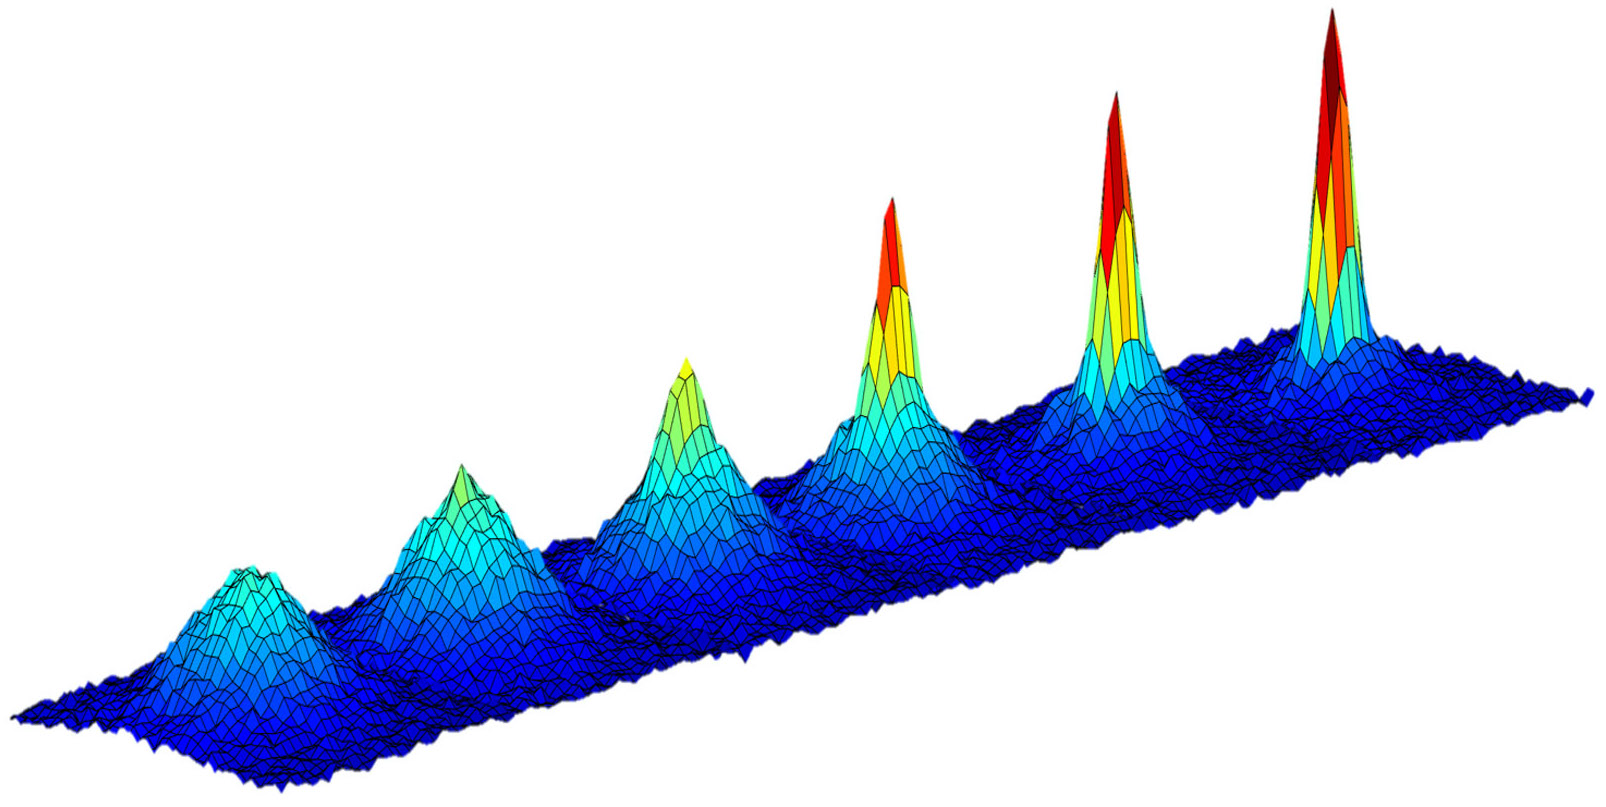
\includegraphics[width=0.7\textwidth]{figures/bec2}
	\caption{Velocity distribution for a gas of rubidium atoms.\footnotemark \\ 
	This demonstrates the formation of a BEC in great detail.}
\end{figure}
\footnotetext{Source:  \tiny{\url{https://www.jpl.nasa.gov/spaceimages/details.php?id=PIA22561} (23.06.2020)}}
\end{frame}


\begin{frame}{Implications}
\begin{itemize}
	\item In order to reach the expected B-E equilibrium distribution, particle-number decreasing \alert{inelastic} processes must occur.
	\item Two possible equilibrium states: Either a system with a condensate (only elastic collisions) or a system with fewer particles (affected by inelastic collisions).
	\item Dynamical issue depending on many factors, e.\,g. production/annihilation rates.
\end{itemize}
\end{frame}

\begin{frame}{Kinetic Evolution dominated by Elastic Collisions III}
\begin{itemize}
	\item Consider the \alert{transport eqn.}
	\begin{equation}
		\partial_t\hspace{0.1em} f\hspace{0.1em}(\mathbf{k},X) = C_{\mathbf{k}}[\hspace{0.1em}f\hspace{0.1em}],
	\end{equation}
	a simplified version of the \alert{Boltzmann eqn.} (cf. Pavel's talk) without drift terms and the \alert{collision integral} $ C_{\mathbf{k}}[\hspace{0.1em}f\hspace{0.1em}]$ which reads
	\begin{equation}
		\eval{\partial_t\hspace{0.1em} f\hspace{0.2em}}_{\mathrm{coll}} \sim \frac{\Lambda_{\mathrm{s}}\Lambda}{p^2}\partial_p\left\{p^2\left[\frac{\partial f}{\partial p} + \frac{\alpha_{\mathrm{s}}}{\Lambda_{\mathrm{s}}}f\hspace{0.1em}(p)(1+f\hspace{0.1em}(p))\right]\right\}
	\end{equation}
	in the small-angle approximation.
	\item The two relevant scales $\Lambda_{\mathrm{s}}$ and $\Lambda$ are used to compute the \alert{thermalization time} defined by the relation $\Lambda_{\mathrm{s}}/\Lambda\sim\alpha_{\mathrm{s}}$.
	\item Taking moments of the collision integral one finds:
	\begin{equation}
		t_{\mathrm{scat}} = \frac{\Lambda\phantom{.}}{\Lambda_{\mathrm{s}}^2} \sim t
	\end{equation}
\end{itemize}
\end{frame}
%TODO: Explain the Lambdas (oral, take some notes)

\begin{frame}{Kinetic Evolution dominated by Elastic Collisions IV}
\begin{itemize}
	\item The integrals are dominated by the largest momenta $\sim \Lambda$. This allows us to approximate the distribution function $f\hspace{0.1em}(p)\sim \Lambda_{\mathrm{s}}/(\alpha_{\mathrm{s}}p)$ up to a cutoff $\Lambda$.
	\item This leaves us with:
	\begin{align}
		n_{\mathrm{g}} &\sim \frac{1}{\alpha_{\mathrm{s}}}\Lambda^2\Lambda_{\mathrm{s}} \\
		\varepsilon_{\mathrm{g}} &\sim \frac{1}{\alpha_{\mathrm{s}}}\Lambda^3\Lambda_{\mathrm{s}}\\
		\varepsilon_{\mathrm{c}} &\sim n_{\mathrm{c}}\cdot m \sim n_{\mathrm{c}}\cdot\sqrt{\Lambda_{\mathrm{s}}\Lambda}
	\end{align}
	with the total number density $n = n_{\mathrm{g}} + n_{\mathrm{c}}$.
	\item Assuming \alert{energy conservation}, i.\,e. $\Lambda_{\mathrm{s}}\Lambda^3\sim \mathrm{const.}$ we can compute the time-dependence of the two scales and therefore the \alert{thermalization time}.
\end{itemize}
\end{frame}

\begin{frame}{Kinetic Evolution dominated by Elastic Collisions V}
From the considerations made before, we determine the time evolution of the scales:
\begin{align}
	\Lambda_{\mathrm{s}} &\sim  Q_{\mathrm{s}}\left(\frac{t_0}{t}\right)^{\frac{3}{7}} \\
	\Lambda &\sim  Q_{\mathrm{s}}\left(\frac{t}{t_0}\right)^{\frac{1}{7}}
\end{align}
and we can confirm that the energy carried by the condensate remains negligible:
\begin{equation}
	\frac{\varepsilon_{\mathrm{c}}}{\varepsilon_{\mathrm{g}}} \sim \left(\frac{t_0}{t}\right)^{\frac{1}{7}}
\end{equation}
Now, we have computed all dependencies to find the estimated \alert{thermalization time} for $\Lambda_{\mathrm{s}}\sim\alpha_{\mathrm{s}}\Lambda$:
\begin{equation}
	t_{\mathrm{th}} \sim \frac{1}{Q_{\mathrm{s}}}\left(\frac{1}{\alpha_{\mathrm{s}}}\right)^{\frac{7}{4}}
\end{equation}
\end{frame}

